\documentclass[12pt]{report}
\usepackage{graphicx, float, algorithm2e}
\usepackage[export]{adjustbox}

\title{\centering CSL351: Analysis and Design of Algorithms \\Assignment No. 1}
\author{\LARGE Sahil\\2016UCS0008}

% to use proper section numbering in the report type 
\renewcommand{\thesection}{\arabic{section}}

\begin{document}

\maketitle

%%%%%%%%%%%%%%%%%%%%%%%%%%%%%%%%%%%%%%%%%%%%%%%%
\section{Problem 1: Water-Jug problem:}

%%%%%%%%%%%%%%%%%%%%%%%%%%%%%%%%%%%%%%%%%%%%%%%%
\section{Problem 2: Euclid's Game:}
In this game, intially there are two unequal numbers written on the board. There are two players, which take alternate turns. In each turn, a player has to write a positive number which is the difference of two numbers on the board, provided \textbf{this new number must not be already present on the board}. The player who cannot make a move loses the game. 
\\ \\ 
To decide on the strategy whether to play first or second, we need to first understand what numbers will be written on the board. If we know the maximum number of new numbers which can be written on the board, then if they are odd, then its better to move first (since the last turn would be even and the 2nd player won't have a move), and if they are even, then its better to move second. 
\\ \\
Suppose the numbers are $a$ and $b$ where $a > b$, then, the first new number $= a - b$, Now, if $a - b > b$, then the second new number will be $a - 2b$ otherwise $2b - a$, Continuing in this way, we can see that the numbers must be some linear combination of $a$ and $b$, i.e. $x*a + y*b$, where  $a$ and $b$ are integers such that $x*a + y*b > 0$.
\\ \\
If we are somehow able to find the smallest possible positive number which can be written as this linear combination, then we can easily know the new numbers which will be written on the board. 
\\ \\
We know that if a number $x$ divides two numbers $a$ and $b$, then $x$ must divide linear combination of $a$ and $b$ also, so consider the \textbf{gcd(a, b)}. Let 
\[ d = gcd(a, b) \]
Then, $d$ divides all the linear combinations of $a$ and $b$, and it must be the smallest such linear combination since if $p$ divides $q$, then $ p \leq q$. 
This can be proved in a more rigorous manner.
\\ \\ 
Now, we know that all the numbers written on the board till the end will be multiples of $\textbf{d}=$ \textbf{gcd(a, b)}. Thus, we can easily count them because we know the maximum multiple of  $d$ written on the board has to be either $a$ or $b$, since we won't generate higher numbers than them. Thus, numbers on the board after end of game = 
\[\frac{max(a, b)}{gcd(a, b)} - 2\]
Here, we are subtracting 2 since they are already present in the starting. 
\\ \\
Thus, if the above number comes out to be \textbf{odd}, then its better to move \textbf{first}, otherwise its better to move second.
%%%%%%%%%%%%%%%%%%%%%%%%%%%%%%%%%%%%%%%%%%%%%%%%
\section{Problem 3: Eight-queens problem:}
There can be a total of $8^{8}$ possibilities of placing $8$ queens on a $8x8$ chessboard, since we can have one queen in any of the 8 positions in any column. 
\\
But, we need to identify the no. of positions in which no two queens are in the same row or in the same column or same diagonal. 
\\
We can use the following algorithm to identify the required positions: 
\\ \\
\begin{algorithm}[H]
	\SetAlgoLined
	\For{all positions of queen in first column}{
		\For{all positions of queen in second column}{
			\For{all positions of queen in third column}{
				... (same pattern)\\
				\For{all positions of queen in $8^{th}$ column}{
					checkWhetherSafe(current positions) \;
					// the above function checks whether there exist a \\
					// row, column or diagonal in which \\
					// two queens are present \\
					// if present it returns unsafe
				}
			}	
		}
	}
	\caption{Eight queen problem - Exhaustive search}	
\end{algorithm}
In the above brute force algorithm, we can increment one \textbf{count} variable each time the configuration is marked as safe. We find that 92 such configuration exists.
\\ \\
To estimate the amount of time taken to estimate all the solutions, we need to know the time complexity of the above algorithm. Since we need to check all $8^{8}$ configurations, i.e. $O(n^{n})$ as conveyed by the 8 nested for loops, and the function \textbf{checkWhetherSafe} checks all rows, columns and diagonals, it takes about $O(n^{2})$ operations, thus total complexity is $O(n^{n + 2})$. 
\\ \\
Thus, we can estimate the time to find all solutions on a compute capable of checking $10$ billion instructions per second = 
\[\frac{8^{10}}{10^{9}} = 1.07 \ seconds\]

%%%%%%%%%%%%%%%%%%%%%%%%%%%%%%%%%%%%%%%%%%%%%%%%
\section{Problem 4: Farmer-Goat-Wolf puzzle:}
The problem states that a farmer has to transport a wolf, a goat and a bale of grass to the other side of the river  in his boat, given the condition that the boat can carry the farmer along with one other item. In his absence, the wolf eats the goat and the goat eats the cabbage. 
\\\\
So, we first try to think what possibilities we have in the first step. If the wolf is taken with farmer, the goat eats the cabbage OR if the grass is taken to the other side, the wolf eats the goat. So, the only possibilty we have is to take the goat with the farmer. 
\\\\
Let \textbf{S1} refer to the other side of the river where we need to transport all of them, \& S2 be the current side of the river. 
\\\\
\textbf{After Step 1 : Farmer \& Goat on S1} and \textbf{Wolf, Grass on S2} 
\\\\ 
Now, the farmer should alone go back to S2 as if the goat goes with him back, then it leads us back to the original state.
\\ 
\textbf{After Step 2: Goat on S1} and \textbf{Farmer, Wolf, Grass on S2}
\\\\
Currently, he can take either of Wolf and Grass to S1, let us consider taking Wolf on the other side. 
\\ 
\textbf{After Step 3: Goat, Wolf \& Farmer on S1} and \textbf{Grass on S2}
\\\\
Note that in the presence of the farmer the Wolf can't eat the Goat, so this configuration is perfectly valid. But, we can't go alone to S2, so he has to take either of them back to S2. Let us consider taking Goat back to S2. 
\\
\textbf{After Step 4: Wolf on S1} and \textbf{Farmer, Goat \& Grass on S2}
\\\\
This time he takes grass with him to S1, since Wolf can't eat the grass.
\\
\textbf{After Step 5: Wolf, Grass \& Farmer on S1} and \textbf{Goat on S2}
\\\\
Now, he goes back alone to S2 and brings Goat also to S1 reaching the final state. 
\\
\textbf{After Step 6: Wolf \& Grass on S1} and \textbf{Farmer \& Goat on S2}
\\
\textbf{After Step 7: Wolf, Grass, Farmer \& Goat on S1}. This is the final state we wanted to achieve. 

%%%%%%%%%%%%%%%%%%%%%%%%%%%%%%%%%%%%%%%%%%%%%%%%
\section{Problem 5: Konigsberg bridges puzzle:}
To problem of starting from any point of Konigsberg and returning back to same point by crossing all seven bridges exactly once, can be transformed into a problem of visiting all the edges in the graph exactly once, starting and ending on the same node.
\begin{figure}[H]
	\vspace{0pt}
	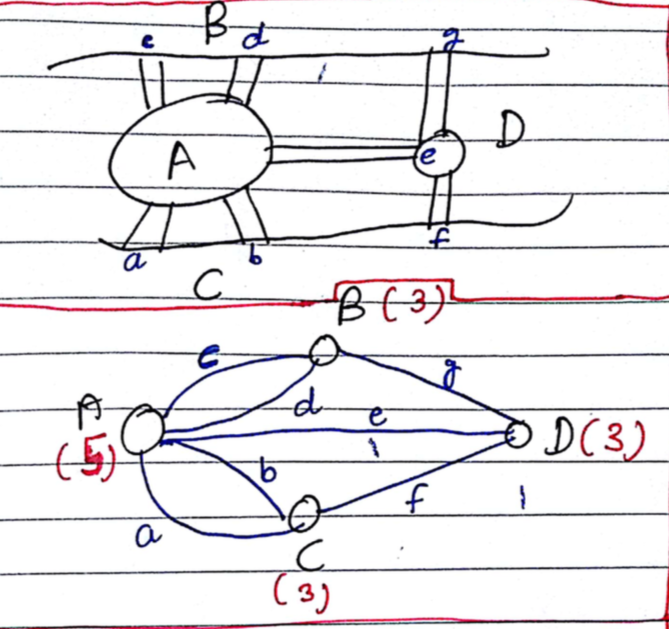
\includegraphics[width=\linewidth, keepaspectratio]{Snapshots/q5_1.png}
\end{figure}  
Now, suppose that we do not have to return back to the same starting point but have to cross all the egdes exactly once, then, let us assume the starting and end points. Now, in between them, whenever we enter a node, we must exit it. So, whenever crossing any node by an edge, it must have 2 unvisited edges, if we do not want to cross the visited edges again. Thus, any node in between the start and end points must have even degree.
That is, there can be exactly 2 nodes with odd degree (start and end) and rest all must have even degree. 
\\ \\ 
But, in this problem, we also want to return to the starting point, this means that, first we can find a path which visits all edges exactly once from start to end as mentioned above, and then we must have another unvisited edge which connects the end point to the start point. Thus, in this case, all the nodes \textbf{must} have \textbf{even degrees}, as in above case only nodes between them had even degrees, but now when we leave from start and reach end, we must have another edge to go from end to start, which makes them also even degree nodes.
\\ \\ 
Since our graph has all nodes with odd degrees, we \textbf{cannot find such a path}.
\\ \\ 
Now, to make such a path possible, we have to add \textbf{minimum} 2 bridges as shown in the following figure. These 2 bridges are highlighted by dark blue color. Adding these two bridges, each between two vertices of odd degree, makes them even degree vertices. 
\\ \\ 
The path is also highlighed, which starts from A and ends on A, taking edges numbered 1 first, 2 then, and so on. 
\begin{figure}[H]
	\vspace{0pt}
	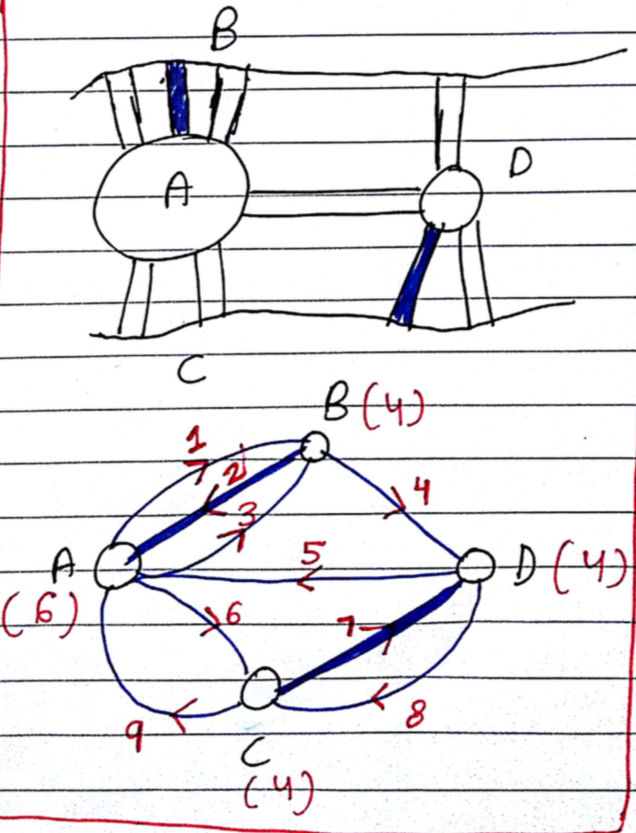
\includegraphics[width=\linewidth, keepaspectratio]{Snapshots/q5_2.png}
\end{figure} 
%%%%%%%%%%%%%%%%%%%%%%%%%%%%%%%%%%%%%%%%%%%%%%%%
\section{Problem 6: Best route for Delhi metro passenger:}
We can model the problem of determining the best route for a metro passenger to take from one station to another as a graph problem where the nodes are the stations and the connections between them are the edges. Since the best route could vary from person to person, it could be either minimum time taking route, minimum cost path or even the one that has least no of stations in between.
\\ \\
For the sake of simplicity, let us consider finding the route that has least no. of stations in between the starting and ending station. We can use a \textbf{breadth first search} kind of approach to find such a route. 
\\ \\

\begin{algorithm}[H]
	\SetAlgoLined
	\For{each station u except starting station s}{
		// set the attributes for each station \\
		$u.visited\gets false$ \;
		$u.distance \gets \infty $ \;
		$u.parent \gets NIL $ \;
	}
	// mark starting station as visited \\
	$s.visited \gets true $ \;
	$s.distance \gets 0 $ \;
	$s.parent \gets NIL $\;
	// create an empty queue for BFS \\
	$Q \gets \phi $ \;
	ENQUEUE(Q, s) \;
	\While{$Q \neq \phi$}{
		u = DEQUEUE(Q) \;
		\For{$each \ v \  \epsilon \ adjaceny \ list \ of \ u$}{
			\If{v.visited equals false}{
				$v.visited \gets true $ \;
				$v.distance \gets u.distance + 1 $ \;
				$v.parent \gets u$ \;
				ENQUEUE(Q, v) \;
			}
		}
	}
	\caption{Find best route for Metro passenger}	
\end{algorithm}

After running BFS as shown, the \textbf{distance} attribute of the destination provides information about the number of stations from the starting point to it, whereas we can get to know about the route by following the \textbf{parent} attributes of the destination, till we reach the source. 
\\
%%%%%%%%%%%%%%%%%%%%%%%%%%%%%%%%%%%%%%%%%%%%%%%%
\section{Problem 7: Door-toggle puzzle:}
There are \textbf{n} doors and initially all of them are closed. On the i-th pass, the door of every i-th switch is toggled. We need to find which doors will be open and which will be closed at the end of n-passes.  
\\ \\
We can write the following \textbf{brute force} algorithm to solve this problem:
\\ \\
\begin{algorithm}[H]
	\SetAlgoLined
	let \textbf{switch} = array of size n initialized with all 0's \; 
	// zero represents closed door and one represents open door \\
	\For{$i\gets 1$ \KwTo $n$}{
		// i represents the current pass, so every i-th door is toggled \\
		$j\gets i$ \;
		// j represents the current door which we increment by i \\
		\While{$j <= n$}{
			// toggle the j-th door \\
			\eIf{switch[j] equals 0}{
				$ switch[j] \gets 1 $
			}{
				$ switch[j] \gets 0 $
			}
			$ j = j + i $
		}
	}
	\caption{Door-toggle puzzle Brute force}	
\end{algorithm}
At the end of the algorithm, we can easily check which doors are open and close by simply looking at the \textbf{switch} array, if the $j^{th}$ entry is 1, that means that door is open, otherwise it is closed.
\\ \\ 
If we run this algorithm, we can observe that all those doors whose numbers are \textbf{prefect squares} will be opened, whereas others will be closed. We can easily prove why this happens. 
\\ \\
\textbf{Claim: } Only those doors whose numbers are perfect squares will be open.
\\
\textbf{Proof: } \\
Let us consider a door numbered $x$. Since at $i^{th}$ pass, we toggle all doors which are multiples of $i$, thus the door $x$ will be toggled only in those passes which are factors of $x$. For eg. door $10$ will be toggled in $1^{st}$, $2^{nd}$, $5^{th}$ and $10^{th}$ passes. 
\\ 
Thus, any door $x$ will be toggled by no. of times equal to the no. of factors of $x$. 
\\ 
And, since all the doors are closed initially, any door which is toggled \textbf{even} no. of times, will remain closed, whereas the one which is toggled \textbf{odd} no. of times will be open at the end. 
\\
We can calculate the no. of factors of any number $x$, if we know its prime factorization. Let:
\[ x = p^{\alpha}.q^{\beta}.\ ...\ .r^{\gamma} \]
where $p$, $q$, ... , $r$ are primes, and $\alpha$, $\beta$, ... , $\gamma$ are positive integers. 
Then, no. of factors of $x$ = 
\[ (1 + \alpha)(1 + \beta)...(1 + \gamma) \]

So, $x$ will have even no. of factors when, either of the multiplication term in above expression is even, i.e. either of $\alpha$, $\beta$,...,$\gamma$ is odd. In other words, it will be odd when none of the terms is even, i.e. all $\alpha$, $\beta$,..., $\gamma$'s are even. 
Since in any \textbf{perfect square no.}, all the powers of the prime numbers in the factorization must be even, thus they always have odd no. of factors. 
\\ \\
Hence, all the doors with perfect square number will be open at the end and the rest will be closed. 
\end{document}
